\documentclass{article}
\usepackage[margin=1.5cm,bottom=2cm]{geometry}
\usepackage{fancyhdr}
\usepackage{graphicx}
\pagestyle{fancy}

\begin{document}
\fancyhead[L]{ 
\includegraphics[width=2cm]{au_logo.png} }
\fancyhead[R]{PHYS 2240: General Physics I}
\fancyfoot[C]{\thepage}
\vspace*{0cm}
\begin{center}
	{\LARGE \textbf{Quiz 1}}
	%\vspace{0.25cm}
	%{\Large Due: Friday, September 11}
\end{center}

A ping pong ball (mass = 3 g), is struck and moves with a speed of 20 m/s to the right and downward at an angle of $30^\circ$ to the vertical. The ball bounces and then moves upward at the same angle and with the same speed. What is the ball's change in momentum (expressed as a vector) during this interaction? \textit{Note: remember to express your answer using SI units!}
\begin{center}
	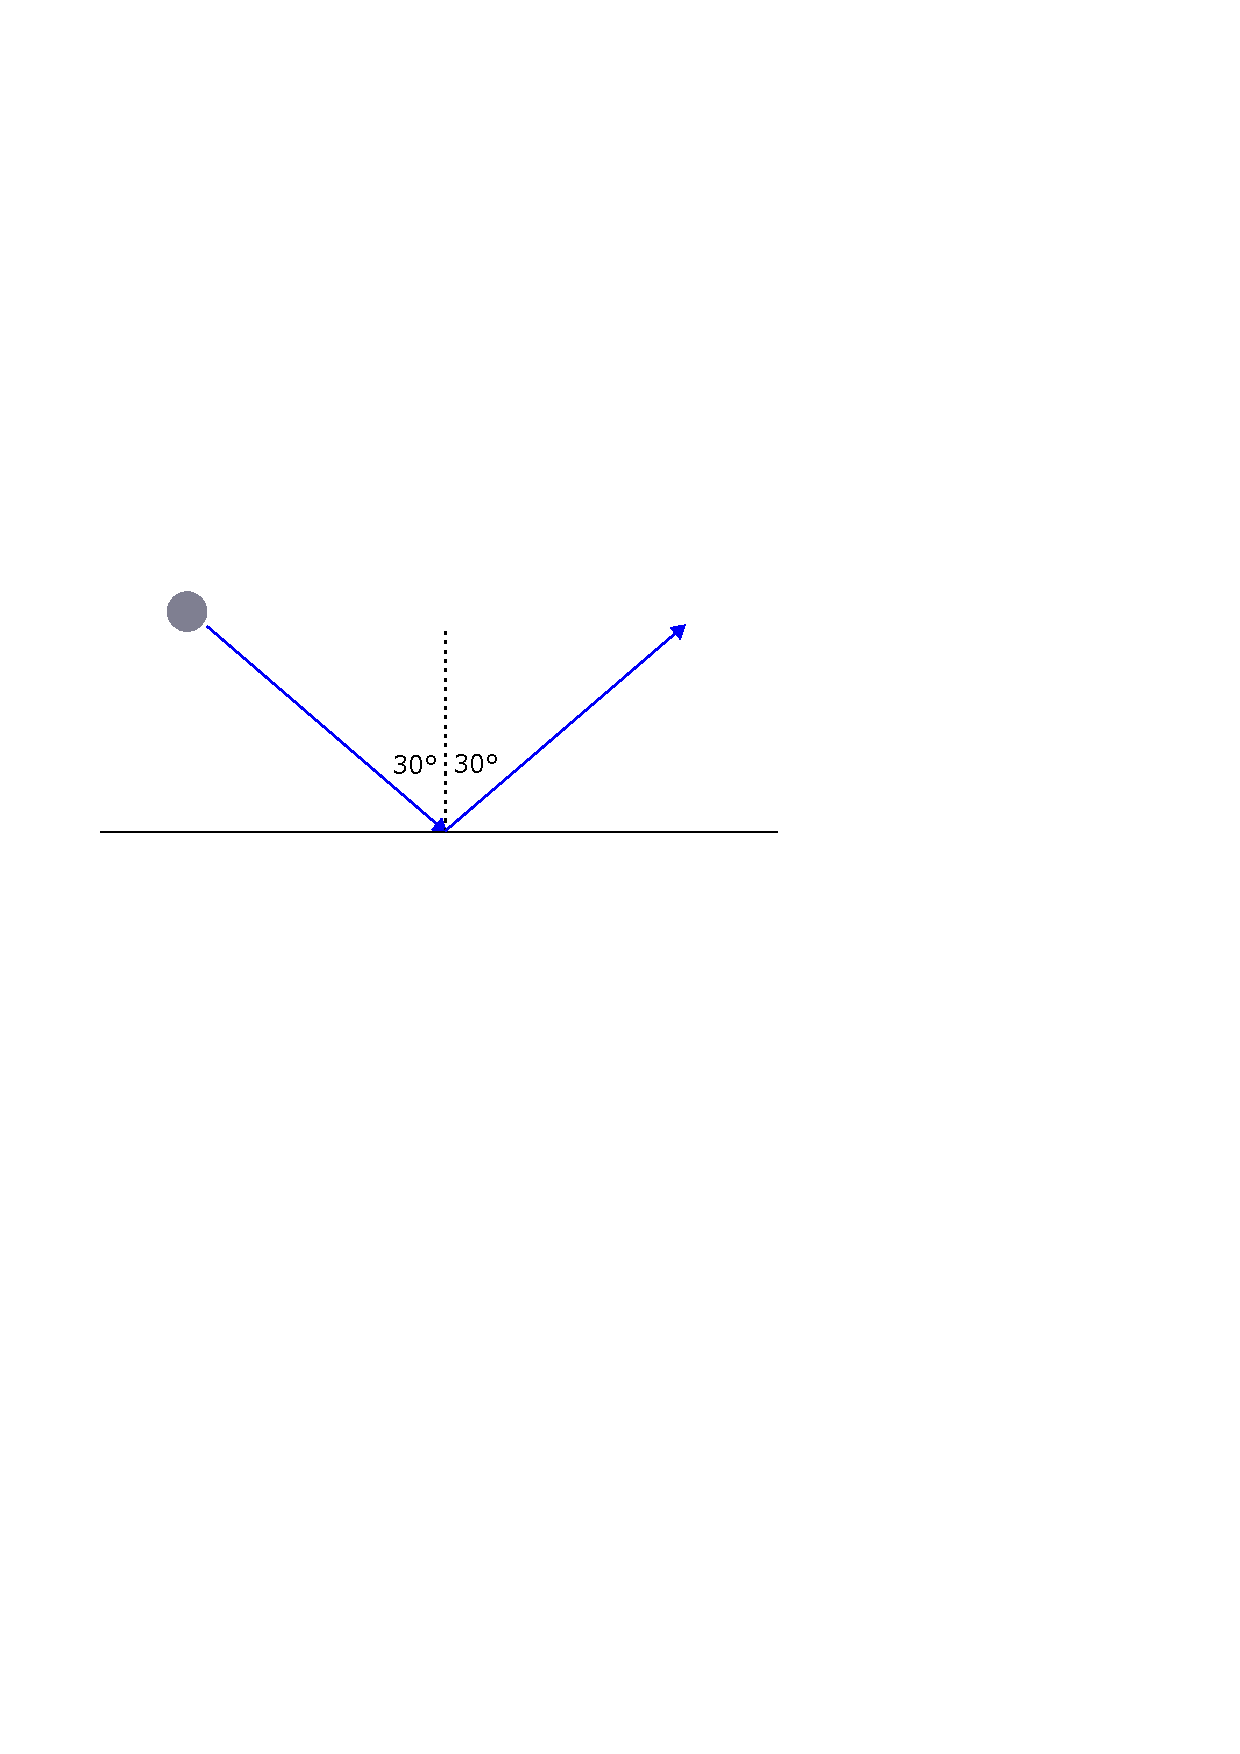
\includegraphics[width=10cm]{quiz1.pdf}
\end{center}

\end{document}